
\section{Our approach}

PPoSS targets large-scale systems and we believe that GPUs will form the backbone of future large-scale, compute-intensive systems. Why?

With power constraints continuing to be the main bottleneck in increased computing performance, the superior power-performance of GPUs~\cite{Dally:2010:GCT} will make them increasingly attractive at all scales, from mobile devices to laptop and desktop computation to the largest supercomputers. The recent and extremely rapid rise of training deep neural networks for deep-learning applications~\cite{Amodei:2015:DS2,Chetlur:2014:CEP,Coates:2013:DLW,Hannun:2014:DSU}---a field led by NVIDIA GPUs and CUDA---has resulted in NVIDIA-GPU-equipped data centers in nearly every large Internet company and NVIDIA GPUs in each of the three major cloud computing providers. As well, GPUs have made enormous inroads into the largest-scale computations. GPU-centered machines dominate the top of the biannual TOP500 list~\cite{top500:nov2022}, including 7 of the top 10 (\#1 and \#3 have AMD GPUs; 157 total of the 168 GPU-centered machines have NVIDIA GPUs). In systems that have high compute requirements, GPU hardware is now ubiquitous.

The most successful GPU applications have historically been focused on highly parallel, regular workloads (e.g., training deep neural networks). What has been more challenging, and the focus of significant research effort over the past decade, has been \emph{irregular} and/or \emph{sparse} workloads that are harder to parallelize effectively. These workloads include the powerful data structures that are the focus of this proposal. While these workloads may exhibit ample parallelism and thus are potentially a good fit for the GPU, they are challenging to implement efficiently because they do not naturally map well to key GPU software design guidelines:

\begin{description}
  \item[Thread divergence] GPUs run most efficiently when neighboring threads take the same path through the code.
  \item[Memory coherence] GPU memory systems are most efficient when neighboring threads access neighboring locations in memory.
  \item[Low contention] Because GPUs have hundreds of thousands of active threads at any time, avoiding memory contention and serialization is critical to allowing GPU threads to progress and thus enabling the GPU to run at maximum efficiency.
\end{description}


Over the past fourteen years, our team has significant experience in developing data structures that address these challenges. We developed the first hash tables that could be built on the GPU~\cite{Alcantara:2009:RPH,Alcantara:2011:BAE} and a plethora of dynamic data structures that were the first to be built on the GPU~\cite{Ashkiani:2018:ADH,Ashkiani:2018:GLA,Awad:2019:EAH,Geil:2018:QFA}. For this proposal, though, more important than the introduction of a new dynamic data structure for GPUs are the big-picture lessons we learned through the process of building all these data structures. These include the utility of warp-wide computation to address thread divergence and memory coherence~\cite{Ashkiani:2017:PAA}; the identification and selection of algorithmic variants to minimize contention~\cite{Awad:2019:EAH}; the use of both coarse- and fine-grained operations to address the variety of challenges inherent in data structure operations; novel approaches to custom memory allocators tailored to particular data structures~\cite{Ashkiani:2018:ADH}; the semantics of bulk data-structure operations; extensions to existing data structures to support snapshots and multi-point queries~\cite{Awad:2022:AGM}; and the importance of real-world workload identification and characterization in building data structures that effectively address actual problems faced by researchers and practitioners. What we learned from these lessons will be vital in ensuring our success with this proposed work.




\subsection{GPUs and High Performance Computing}

PPoSS targets large-scale systems and we believe that GPUs will form the backbone of future large-scale systems. Why?

With power constraints continuing to be the main bottleneck in increased computing performance, the superior power-performance of GPUs~\cite{Dally:2010:GCT} will make them increasingly attractive at all scales, from mobile devices to laptop and desktop computation to the largest supercomputers. Power constraints are also motivating overprovisioned systems where only a subset of the silicon can be powered at any one time. Such systems tilt toward more heterogeneity, further motivating hybrid systems---and an increased need for GPU-focused computation---as the future norm. We believe accelerators such as GPUs will play a fundamental and integral role in next-generation high-performance computing systems.

Accelerators are becoming increasingly popular in supercomputing, with NVIDIA GPUs programmed with CUDA being a popular  choice for scientific application and infrastucture development.  In the commercial world, the recent and extremely rapid rise of deep-learning  applications~\cite{Amodei:2015:DS2,Chetlur:2014:CEP,Coates:2013:DLW,Hannun:2014:DSU} has led to data-center systems designed for the computationally demanding problem of neural net training, currently dominated by NVIDIA GPUs and CUDA\@.  Nearly every Internet company has NVIDIA-based systems for this purpose.

The most common use of the GPU today is as a coprocessor for compute-intensive tasks. The CPU is responsible for the main runtime, which allocates and populates input data in GPU-accessible memory. The CPU then launches kernels on the GPU to process that memory and fetches the results when the GPU completes its processing. GPUs are certainly prominently featured in some of today's largest distributed memory machines---for instance, ORNL's Titan has an equal number of CPUs and GPUs, but the GPUs account for 90\% of its FLOPS\@. However, the way we program these machines is over 20 years old. We can sum this up in one sentence: GPUs are treated as coprocessors and communicate via MPI where the CPU's runtime is preeminent. This coprocessor model is well-suited for workloads that are large and compute-intensive (to amortize control and transfer overheads) with simple control (to allow the GPU to run without CPU intervention), and is exploited by GPU computing libraries. It is, however, a model where the GPU has little autonomy, and as we will discuss in the next sections, a model poorly suited for our future productive and high-performance computing needs.

We believe the time is right to upend this model and make the GPU more of a first-class processor. We are excited about recent advances in the GPU ecosystem that have added significant functionality enabling our proposed research:

\begin{itemize}
\item Driven by a desire to deliver maximum memory bandwidth, we expect to see both more GPUs on a node (e.g., NVIDIA's DGX2 with 16 GPUs) as well as more GPUs per card. The result is a density that makes using GPUs more attractive and less costly.
\item Inter-GPU and CPU-GPU interconnect is making a significant leap in performance, led by NVIDIA's NVLink (bidirectional 80~GB/s) and OpenCAPI~\cite{DeGelas:2016:OUA}.
\item NVIDIA GPUs now support a unified virtual memory space between CPU and GPU, though manual management is still essential for even single-GPU performance on real-world workloads and certainly for multi-GPU machines. In general, NVIDIA's philosophy has been (1) to expose new hardware mechanisms with functional but limited software support; (2) to see how applications use those mechanisms; and then (3) to optimize their software and  hardware to make those application patterns efficient. Our motivation here is clearly to lead the way in the second step.
\item LLVM now features (open-source) NVIDIA GPU support through Google's gpucc compiler effort~\cite{Wu:2016:GAO}. This work enables compiler research on NVIDIA GPUs that was not previously possible.
\end{itemize}

As GPUs have become an integral part of today's supercomputers, the hardware and software support from vendors and researchers alike has moved beyond the basic model of GPUs communicating only with their host CPU through PCI Express and CPU host memory.

\paragraph{Hardware Support via GPU-to-GPU Communication}
\label{sec:gpudirect}

Historically, all network transfers to or from GPUs had to pass through the CPU and its memory system. This was a significant performance obstacle, particularly due to the inefficiency of copies. Before 2010, a network transfer from a GPU required three copies: (1)~GPU to CPU pinned memory; (2)~CPU copy from user space into driver space; (3)~transfer to the NIC\@. Hardware ``GPUDirect'' support was designed to address this inefficiency. In 2010, the first iteration of GPUDirect shared memory access allowed the sharing of pinned memory between the GPU and the network driver, removing the second copy above. Later GPUDirect advances allowed direct peer-to-peer communication between GPUs on the same PCIe bus (``GPUDirect Peer-to-Peer'', 2011) and direct support for GPU-to-remote-GPU RDMA (``GPUDirect Support for RDMA'', 2012) that does not pass through the CPU at all. NVIDIA offers detailed uidelines~\cite{NVIDIA:2022:DAL} to developers who wish to use this technology.

\paragraph{MPI two-sided and collective support for GPUs}

The predominant access to internode communication has been through MPI, with most work on the two-sided and collective features of MPI\@.  Direct GPU capabilities are part of Cray's MPI and the IBM Platform MPI, but the most significant use has been through MVAPICH2 (since version 1.8) and OpenMPI (also since version 1.8). At a lower level, Mellanox's Infiniband software stack provides direct support for RDMA, and of course Mellanox has now been acquired by NVIDIA (2020) and so we expect this network-GPU tie to only deepen. NVIDIA has implemented a high-performance set of collectives within a single node, which are important as nodes become more powerful and application run multiple MPI ranks per node.  ``NCCL'', NVIDIA's accelerated multi-GPU collective communication library~\cite{Luehr:2016:FMC}, implements broadcast, reduce, all-gather and -reduce, and reduce-scatter for multiple GPUs on a single node.  The ``OSU Micro-Benchmarks'' (version 5.8 as of August 2021)~\cite{MVAPICH:2021:OMB} provide a set of comprehensive benchmarks that include CUDA/OpenACC extensions, primarily latency and bandwidth tests that include MPI collectives.

Ernsting and Kuchen's ``Muesli'' library of algorithmic skeletons~\cite{Ernsting:2012:ASF} was built atop MPI, OpenMP, and CUDA\@. And some MPI packages, such as MVPICH2, take advantage of GPUDirect hardware in accelerating MPI operations. These components are solid building blocks for our work. What they collectively lack is any user-programmable runtimes on the GPU side. We believe the new hardware capabilities and emerging software building blocks strongly motivate the development of user-programmable runtimes to manage and control them.

\subsection{Why the GPU, and more broadly, massive parallelism?}

The growing difficulty of increasing single-threaded performance~\cite{Ekman:2005:AIL} has motivated a turn to parallelism~\cite{Asanovic:2006:TLO} as the primary means for continuing performance growth in computing. The GPU has emerged as a major player in this landscape. In contrast to a CPU's emphasis on minimizing the latency of a single thread, GPUs instead aim to maximize the throughput of all threads.

\begin{figure}
  \centering
  \begin{tabular}{ccc}
    \includegraphics[width=0.3\textwidth]{figures/deerhound-marked-up} &
    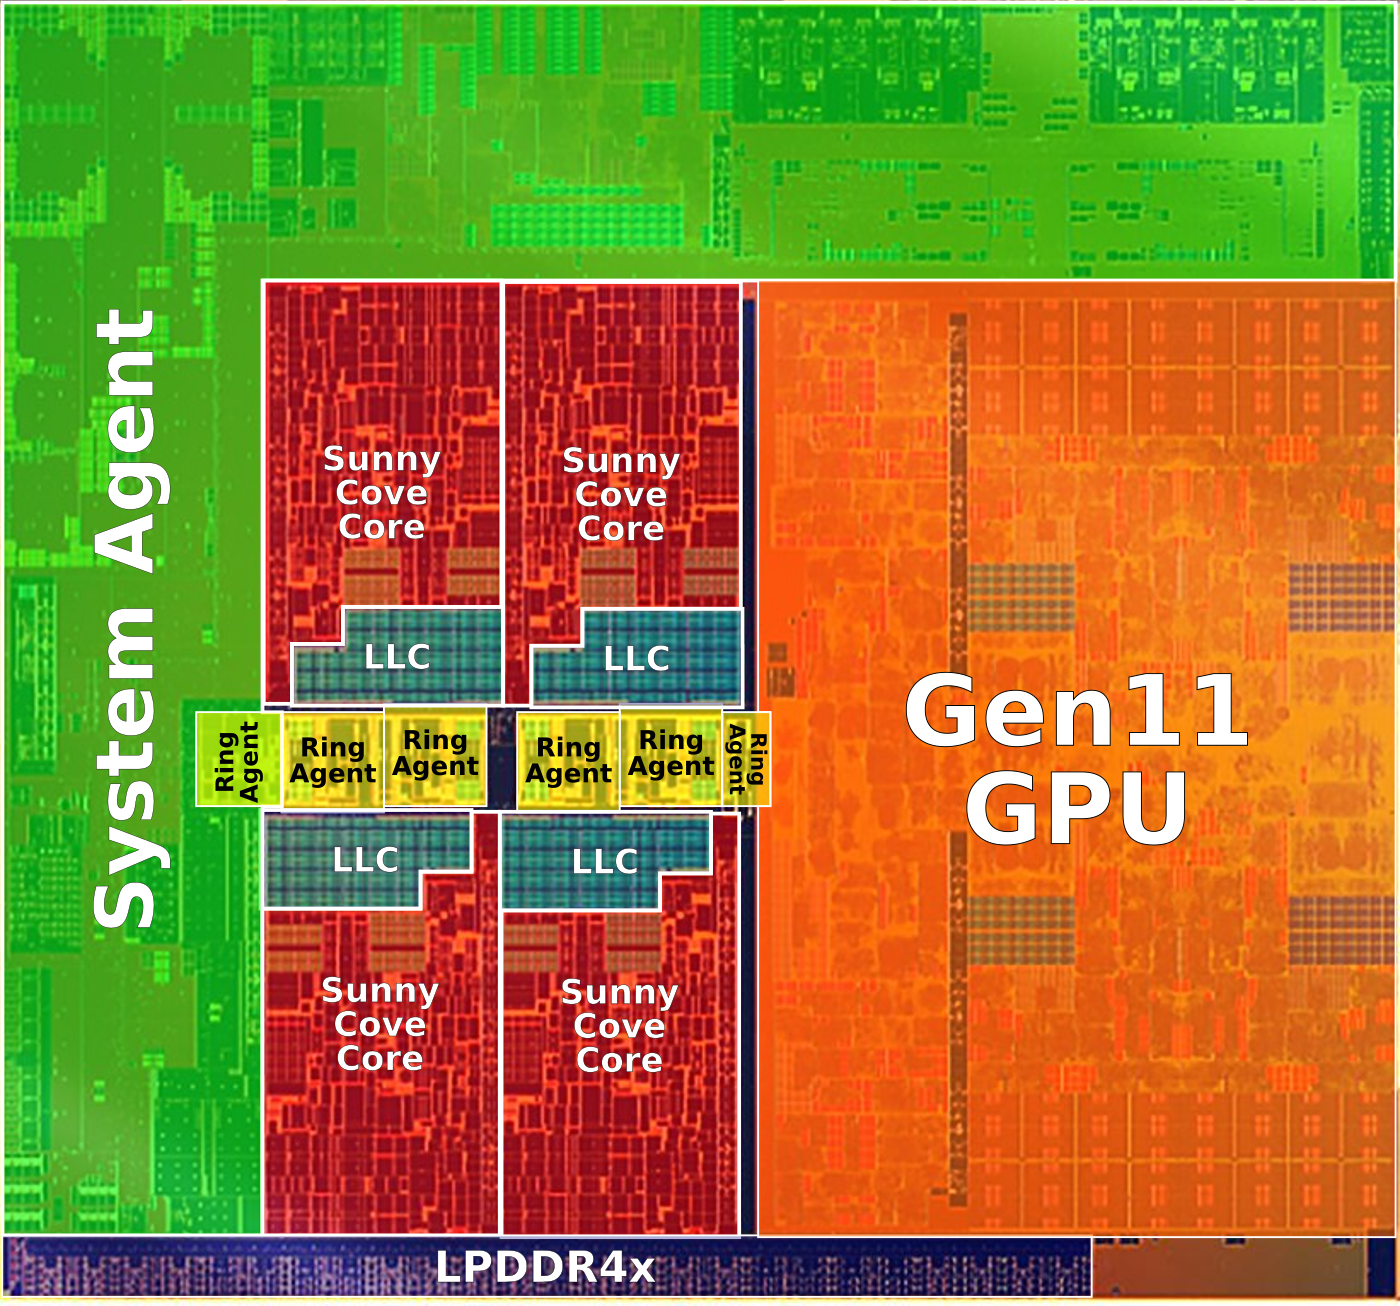
\includegraphics[width=0.3\textwidth]{figures/ice_lake_die_(quad_core)_(annotated)}
  \end{tabular}
  \caption{Over the past fifteen years, the highest-performance computation resources in a mainstream microprocessor have shifted from a small fraction of die area on the CPU to a much larger fraction in an integrated GPU\@. Left: one core of AMD's K8L ``Deerhound'' CPU (2006). Heavy white boxes mark the compute units. Right: Intel Ice Lake hybrid CPU-GPU (2019). Intel's GPU is not only capable of 3D graphics but also general-purpose compute through interfaces like OpenCL\@. \label{fig:gpus-on-modern-processors}} \end{figure}

By focusing on throughput, GPU vendors build designs that are well-suited to address today's most important technology trends. Modern VLSI gives us an increasing number of transistors but little to no increase in clock speeds; GPU vendors have built hardware and software that together scale well with more, rather than faster, hardware resources. The gap (``memory wall'') between processor capability and memory bandwidth continues to grow; throughput-oriented processors like GPUs are designed to amortize increasing memory latency by quickly context-switching to other parallel work. And in a power-constrained world, GPUs have a significant advantage; in his 2010 Supercomputing keynote, Dally cited contemporary figures of 200~pJ/instruction for GPUs and 2~nJ/instruction for CPUs~\cite{Dally:2010:GCT}, with the GPU's power efficiency advantage changing little over the past decade~\cite{Dally:2020:DHA}. It is thus no surprise that even CPU vendors are increasingly emphasizing GPU-like cores on their most recent processors (Figure~\ref{fig:gpus-on-modern-processors}).

With power constraints continuing to be the main bottleneck in increased performance, the superior power-performance of GPUs will make them increasingly attractive. Power constraints are also motivating overprovisioned systems, particularly systems-on-a-chip, where only a subset of the silicon can be powered at any one time~\cite{Esmaeilzadeh:2011:DSA}. Such systems tilt toward more heterogeneity, further motivating hybrid systems---and an increased need for the more energy-efficient GPU-focused computation---as the future norm.
% https://www.nextplatform.com/2022/11/14/testing-the-mettle-of-the-top-supercomputing-iron-on-earth/

But, the front-and-center reason for a continued focus on GPU graph analytics today is outside the scope of graph analytics entirely. The new reality is:

\begin{itemize}
  \item The recent and extremely rapid rise of training deep neural networks for deep-learning applications~\cite{Amodei:2015:DS2,Chetlur:2014:CEP,Coates:2013:DLW,Hannun:2014:DSU}---a field led by NVIDIA GPUs and CUDA---has resulted in NVIDIA-GPU-equipped data centers in nearly every large Internet company and NVIDIA GPUs in each of the three major cloud computing providers. As well, GPUs have made enormous inroads into the largest-scale computations. GPU-centered machines dominate the top of the biannual TOP500 list~\cite{top500:nov2022}, including 7 of the top 10 (\#1 and \#3 have AMD GPUs; 157 total of the 168 GPU-centered machines have NVIDIA GPUs). In systems that have high compute requirements, GPU hardware is now ubiquitous.
  \item Moving data to and from GPUs remains, and appears likely to remain, expensive. Because machine learning and scientific computation are primarily performed today on GPUs, we see an accelerating focus toward ensuring that entire computational pipelines of interest are also on GPUs, to avoid this communication cost. (As an example, it is faster to perform an entire Gunrock breadth-first search on a graph than to transfer that graph between CPU and GPU\@.) So, even if GPU graph applications ran only equally fast as their CPU equivalents, they still offer significant value because they enable faster execution of entire workloads.
\end{itemize}

As a consequence of these two broad trends, NVIDIA has made a large investment into its open-source data science framework, RAPIDS, which has already integrated Gunrock into its codebase and releases, and which will allow us to immediately bring the results from this proposal into widespread use.

%%% Local Variables:
%%% mode: latex
%%% TeX-master: "proposal"
%%% End:


%%% Local Variables:
%%% mode: latex
%%% TeX-master: "main"
%%% End:
